\chapter{Evaluation Methodology}
\label{sec:evaluation}
\ifpdf
    \graphicspath{{6_evaluation/figures/PNG/}{6_evaluation/figures/PDF/}{6_evaluation/figures/}}
\else
    \graphicspath{{6_evaluation/figures/EPS/}{6_evaluation/figures/}}
\fi

The selected timeslices had between 500 to 1692 event hits to capture a variety of event sizes for training. Figure \ref{fig:7_tree} shows the directory structure for the dataset. Timeslices were organised by classes and separated into individual \texttt{training} and \texttt{testing} folders as required by PointNet.

\begin{figure}[ht!]
    \centering
    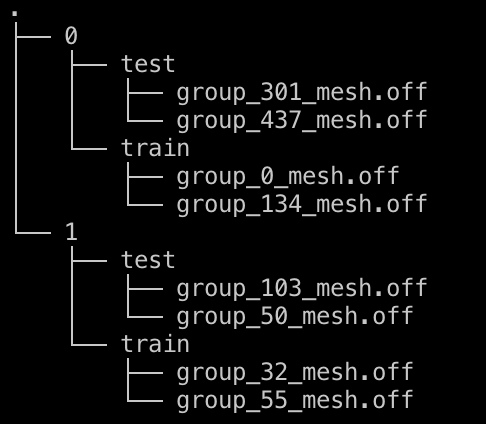
\includegraphics[width=0.4\textwidth, height=5.5cm, keepaspectratio]{tree}
    \caption{Required Directory Structure for PointNet}
    \label{fig:7_tree}
\end{figure}

An 80-20 train-test split was used to randomly select 80\% of the files under each class for training and 20\% for testing. No validation set was required because there was no need to choose an appropriate model from rivalling approaches \cite{dixon2017deep, james2013introduction}. This chapter discusses the preparation of the training and testing data, along with two chosen edge cases. The chapter also describes the ensemble methodology used for obtaining final predictions and remarks on the use of L1 trigger on the dataset for comparison against PointNet.

\section{Training and Testing Data}
\label{sec:eval_train_test_data}
160 timeslices were selected for each class as training data. Both classes had meshes with approximately 4800 vertices on average, and 8500 triangles. A total of 40 timeslices were selected as testing data for each class. Both classes had meshes with approximately 4800 vertices on average and 7500 triangles. The testing data represented much of what the detector would gather in real world, and send to the pipeline for processing. However, two additional edge cases were chosen to evaluate the extent of the model's learning capacity. Most event timeslices have around 700 event hits on average. Therefore, a timeslice with 100 event hits and 6796 noise hits was selected. As an extreme case, a group with 39 event hits and 6645 noise hits was selected.

\begin{figure}[ht!]   
\centering
\subfloat[3D Mesh of Timeslice with 100 Event Hits]{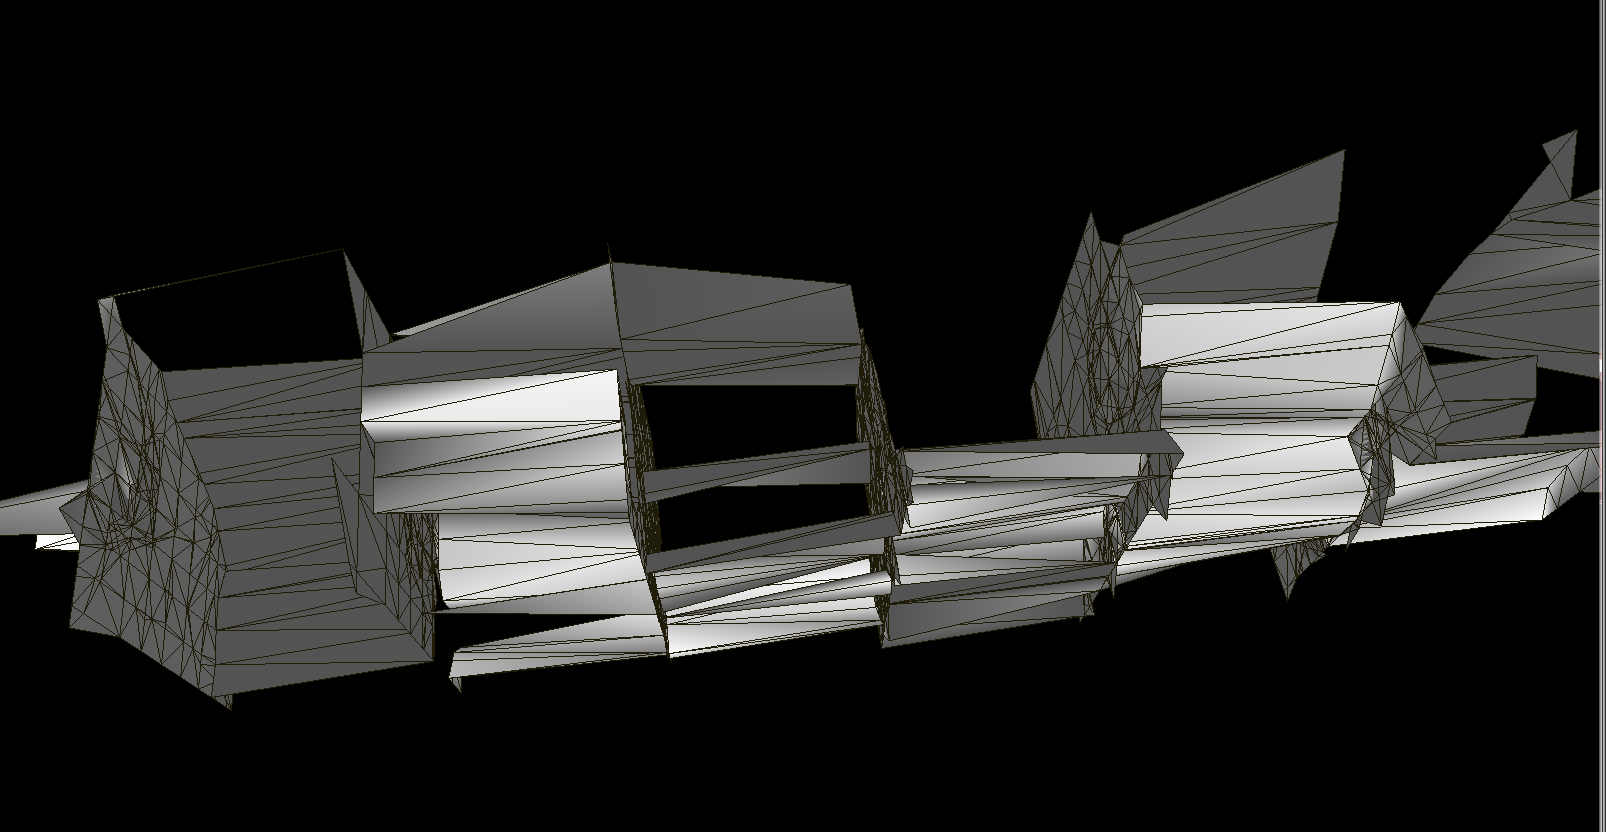
\includegraphics[width=0.49\textwidth, height=6cm, keepaspectratio]{1063.png}\label{fig:1063-mesh}}

\subfloat[Typical Example of Timeslice with Event Hits]{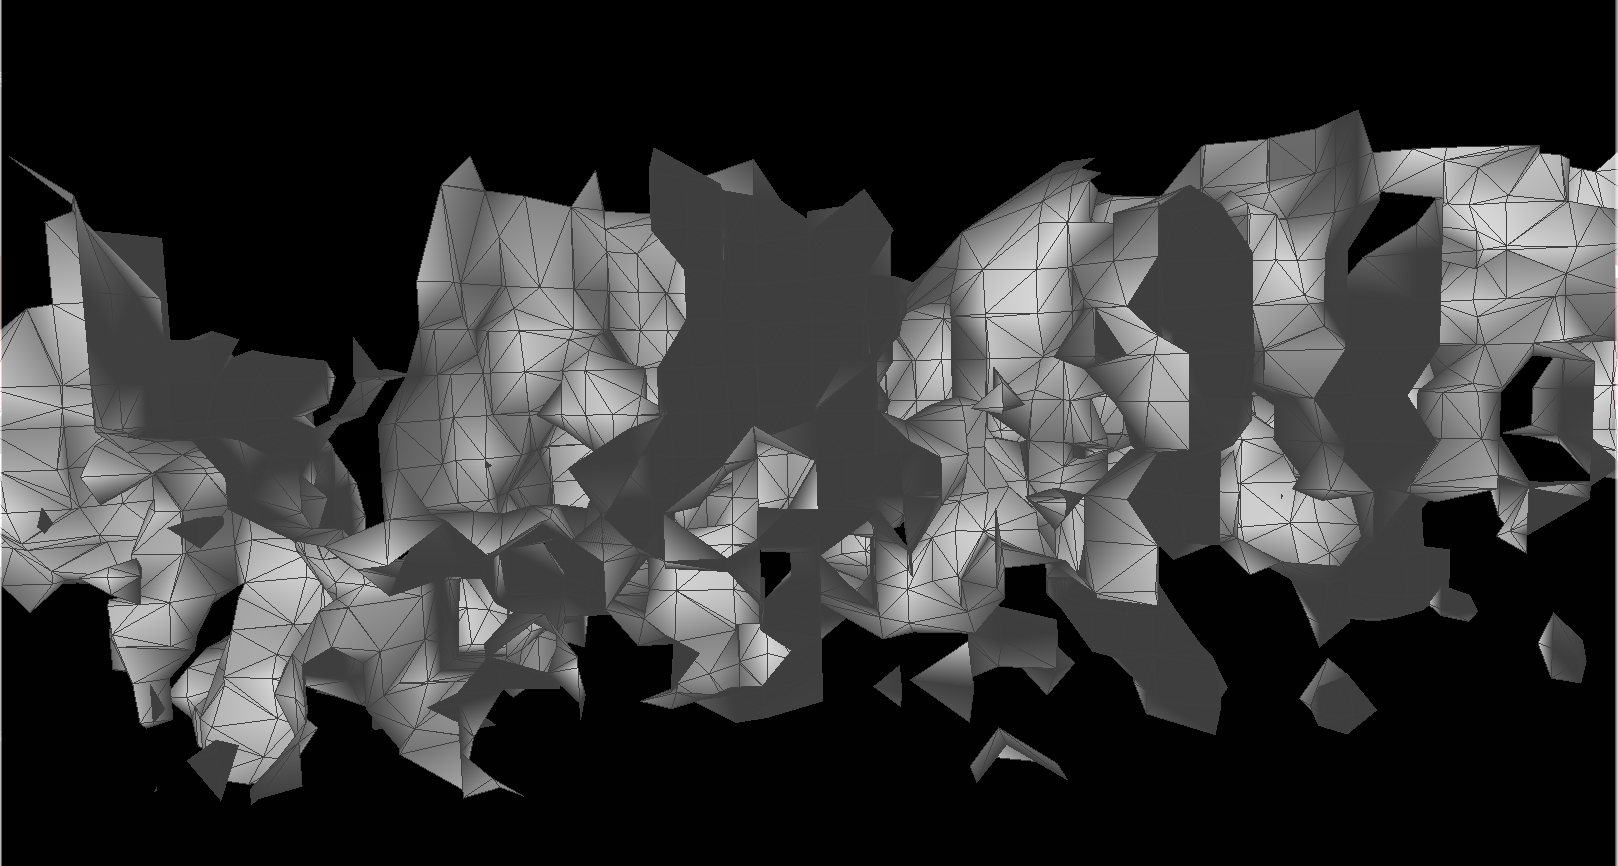
\includegraphics[width=0.49\textwidth,height=3.7cm]{615.png}\label{fig:615-mesh}}
\hspace{0.01cm}
\subfloat[Typical Example of Timeslice with Noise]{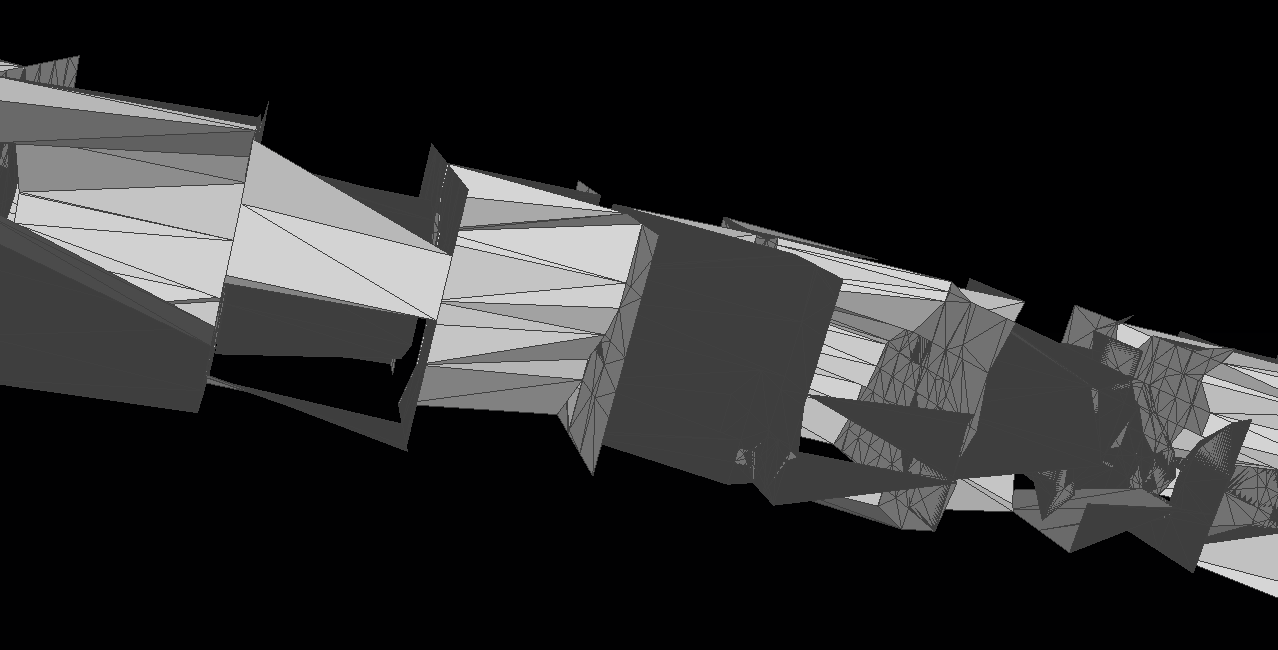
\includegraphics[width=0.49\textwidth,height=6cm, keepaspectratio]{noise.png}\label{fig:noise-mesh}}
\caption[]{Edge Case: Comparison of Mesh Detail for Timeslices with Low Event Hits}
\label{fig:1063}
\end{figure}

Figure \ref{fig:1063-mesh} shows the detail captured by the mesh for a processed point cloud with 100 event hits.
Figure \ref{fig:615-mesh} on the other hand is an example of a typical event cluster rendered with details and rounded surfaces. Figure \ref{fig:noise-mesh} is an example of a typical noise region, rendered as smoother surfaces by Surface Poisson Reconstruction. Figure \ref{fig:1063-mesh} resembles the noise point cloud in Figure \ref{fig:noise-mesh} with smooth surfaces. This indicated that the event hits details were lost in conversion and PointNet may not be able to classify it as an event timeslice. 

Similarly, Figure \ref{fig:5686} shows another example of a point cloud with 39 event hits. The mesh representation contains very few distinguishing features and flat surfaces, unlike a typical event cluster mesh (Figure \ref{fig:615-mesh}). Since the event cluster resembled the mesh representing noise hits, it was likely that PointNet would not be able to classify it as an events class.

\begin{figure}[ht!]
    \centering
    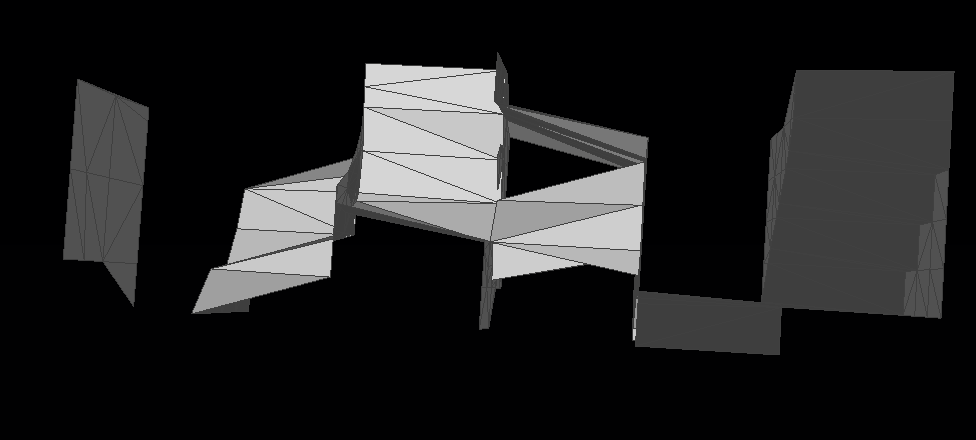
\includegraphics[trim={1cm 1cm 0.5cm 0.5cm}, clip,width=0.7\linewidth,keepaspectratio]{5686.png}
    \caption{3D Mesh of Timeslice with 39 Event Hits}
    \label{fig:5686}
\end{figure}

\section{Model Specifications}
The model was first run for \texttt{200} epochs to find the optimal training epoch value. Figure \ref{fig:epochs} shows that the loss settled around 100 to 120 epochs. Therefore, the rest of the experiments were conducted for \texttt{120} epochs. The loss was found to be between \texttt{0.008} and \texttt{0.003} during training and considered sufficient for the thesis. 

\begin{figure}[ht!]
    \centering
    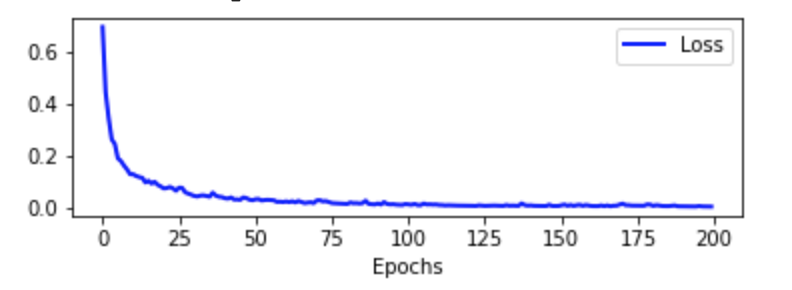
\includegraphics[trim={0 0 0 0.3cm}, clip, width=0.7\linewidth,keepaspectratio]{epochs}
    \caption{Loss Plotted for 200 Training Epochs}
    \label{fig:epochs}
\end{figure}

Model parameters were experimented to obtain optimal performance, but it was noted that the default parameters in the paper by Qi et al. (2017) were best suited for the dataset \cite{qi2017pointnet} (Appendix \ref{appendix-layers}). Table \ref{tab:model_parameters} shows the parameters used for training. For each batch, the model was evaluated on the testing data to obtain a signal about the model's ability to generalise. The dataset was trained with PyTorch using Google Colab NVIDIA Tesla K80 GPU and on ViltStift AMD MI50 GPUs for approximately 3.5 hours.

\begin{table} [ht!]
    \centering
    \begin{tabular}{l c}
    \hline
        regularisation loss with weight & 0.001  \\
        Initial Learning Rate & 0.001 \\
        Dropout probability & 0.3 \\
        Batch Size Training & 32 \\
        Batch Size Testing & 64 \\
        Epochs & 120\\
    \hline
    \end{tabular}
    \caption{Final Model Parameters Used for Training on KM3NeT Data}
    \label{tab:model_parameters}
\end{table}

 
\section{Ensemble Methods for Results}
As \texttt{x, y, z,} and \texttt{time} variables were split into three permutations of (\texttt{x, y, time}), (\texttt{x, z, time}) and (\texttt{ y, z, time}), each dataset was trained separately. The results from each of these datasets were then combined using majority voting ensemble techniques \cite{goodfellow2016convolutional}. Voting ensembles were selected as a suitable methodology for two main reasons. First, while there were three datasets, they represented the same information, except in slightly different manner. Majority voting ensembles place equal value on the models being combined to make predictions which was relevant in this case \cite{bhowan2012evolving}. Second, a voting ensemble is considered appropriate when no single model performs comparatively worse or better than the others \cite{bhowan2012evolving}. Results showed that two of the three models were quite similar in performance.

Two voting ensemble techniques were used to generate the final predictions - hard voting and soft voting. A hard voting ensemble sums the votes for class labels from all models and presents the class with the most vote as the final prediction \cite{witten2002data}. A soft voting ensemble sums the predicted probabilities for class labels and presents the label with the highest sum probability \cite{witten2002data}. A soft voting ensemble additionally requires a probability threshold to finalise the label as positive. A high threshold of 90\% was used due to the physics requirement of minimising false positives and correctly classifying event timeslices as much as possible.

The existing L1 trigger (Section \ref{sec:intro-trigger}) was also applied on the dataset. The results from the L1 trigger were contrasted against PointNet to identify if any improvements could be noted. The L1 trigger is known to save noise timeslices as relevant, so PointNet would have to perform better in that instance. The training and testing data was therefore prepared to ensure that a good range of event sizes were covered. Further, two edge cases for event timeslices were also prepared to establish the extent of the network's learning capacity. Majority voting ensemble was seen as a robust, simple ensemble technique and used to obtain final predictions.

